%!TEX root = volumeFinal.tex 
\chapter{\label{chap:agentes}Agentes} 

Os agentes são utilizados em jogos como uma abstração que represente os jogadores. Agentes conseguem absorver informações providas do jogo e assim decidir qual o próximo passo a ser tomado \cite{millington2009artificial}. \frm[color = yellow]{Explica para o leitor por que tu estás começando por agentes (dica, esta é a abstração usada para pensar em jogos...)}

Formalmente, agentes são entidades que agem de forma continua e autônoma em um ambiente \cite{agent1993oriented}. 
Os agentes são capazes de receber estímulos do ambiente através de sensores, e assim responder aos estímulos por intermédio de atuadores. 
Para os agentes os estímulos do ambiente são recebidos como percepções. 
Os atuadores por sua vez, geram, uma ação considerando as percepções \cite{intelligence2003modern}. 
A interação de um agente com o ambiente pode ser ilustrado pela Figura~\ref{fig:agente}.

%\frm[inline]{Figura, Tabela, Algoritmo, quando em uma referência, sempre em maiúsculo. A definição não é \textbf{representada} pela figura de jeito nenhum. Talvez ilustre o funcionamento de um agente que segue esta definição. Cuidado com este tipo de afirmação.}

\begin{figure}[ht]
	\centering
	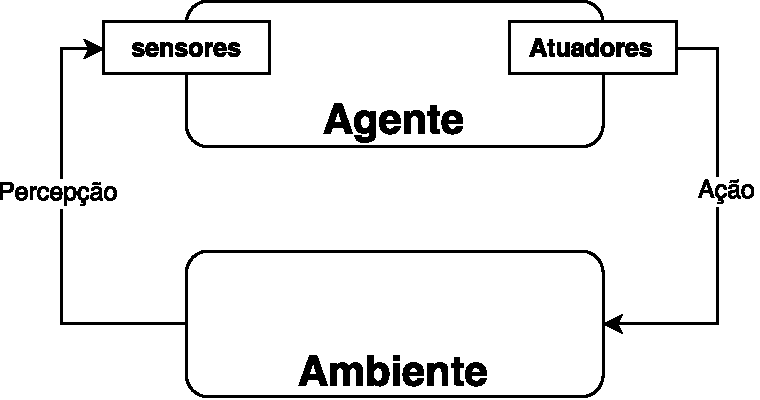
\includegraphics[width=0.5\textwidth]{fig/agente.pdf}
	\caption{Representação de um agente}
	\label{fig:agente}
\end{figure} 

O agente deve agir de forma autônoma, para isso ele deve ser capaz de aprender a lidar com situações proporcionadas pelo ambiente, com o intuito de realizar ações em busca do seu objetivo. O agente precisa de três características para conseguir ser autônomo \cite{agent1999}. São elas:
 
\begin{itemize}
	\item reatividade, para que os agentes sejam capazes de perceber o ambiente e suas mudanças a fim de levar o ambiente em consideração para a tomada de decisão das ações;
	\item pró-atividade, para que os agentes consigam ter a iniciativa em tomar as suas ações; e
	\item habilidade social, para que os agentes sejam capazes de interagir com outros agentes(humanos ou não).
\end{itemize}

As duas primeiras características são necessárias para que o agente consiga interagir com o ambiente. Um agente sendo reativo, ele consegue, a partir de uma mudança do ambiente, saber como ele deve se comportar. Sendo proativo, o agente pode antecipar suas ações em busca do seu objetivo.
Já a terceira característica é necessária para que o agente consiga interagir com outros agentes quando há mais de um agente no sistema. Nem sempre um agente vai estar sozinho no ambiente, sistemas onde existem mais de um agente são chamados de sistema multi agentes. Nesses sistemas, os agentes interagem entre si, podendo ter objetivos em comum ou não. Sendo assim eles terão que cooperar ou negociar entre si \cite{intelligence2003modern}.

\section{Ambientes}

O agente deve se comunicar com um ambiente para conseguir alcançar seus objetivos. Mas um ambiente é composto por diversas propriedades que podem influenciar como o agente vai agir para chegar ao seu objetivo \cite{intelligence2003modern}. 

Nem sempre todas as informações do ambiente estarão disponíveis, por esse motivo o ambiente pode ser dito como completamente observável, parcialmente observável ou não observável, dependendo da informação disponibilizada. Um ambiente é dito completamente observável se, em qualquer instante de tempo, todas as informações relevantes do ambiente estão disponíveis para os sensores do agente. Caso haja alguma informação que não possa ser acessada, em algum instante de tempo, seja por causa da incapacidade do sensor do agente de captar essas informações ou essa informação simplesmente não é disponibilizada, o ambiente é dito parcialmente observável. Agora, se o ambiente não disponibiliza nenhuma informação, o ambiente é tido como não observável \cite{ intelligence2003modern, agent1999}.   

Após o agente realizar uma ação ocorre uma modificação no ambiente. O ambiente é determinístico se o estado gerado após a execução de uma ação, em todas as vezes que for executada, levar para o mesmo estado resultante, ou seja, o estado resultante é determinado pelo estado atual e a ação executada pelo agente. Se não há a certeza do estado resultante, o ambiente é estocástico. Quando o ambiente é não determinístico existem chances das ações levarem para os estados \cite{intelligence2003modern}. 

Os estados do ambiente irão mudar ao longo do tempo, seja por uma ação feita por algum agente, ou por alguma mudança que possa ocorrer em razão de outro processo do ambiente. Se o ambiente sofre alguma alteração apenas quando o agente executa alguma ação, o ambiente é estático. Se o ambiente tem a capacidade de mudar independente de uma ação de um agente, o ambiente é dinâmico \cite{agent1999}.

Em sistemas multi agentes os agentes podem estar competindo ou cooperando entre si. O ambiente é competitivo quando os agentes estão competindo, como em um jogo de xadrez, por exemplo, ou o ambiente é cooperativo quando os agentes estão cooperando \cite{intelligence2003modern}.

\section{Arquiteturas de Agentes}


O tipo mais simples de agente é aquele que apenas reage a uma percepção vinda do ambiente. O agente escolhe suas ações baseado no que percebe no momento da decisão, sem levar em consideração ações já tomadas ou percepções anteriores. O agente apenas responde a uma percepção com uma ação, como se houvesse um clausula de condição, por exemplo, se estiver chovendo eu irei levar um guarda-chuva. A Figura~\ref{fig:agenteSimple} ilustra essa arquitetura. 

\begin{figure}[ht]
	\centering
	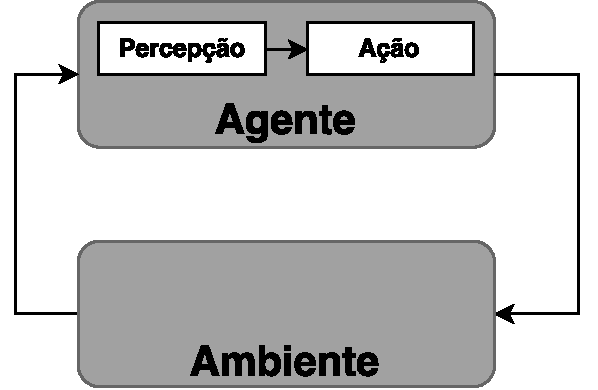
\includegraphics[width=0.4\textwidth]{fig/agentSimple.pdf}
	\caption{Arquitetura simples de um agente.}
	\label{fig:agenteSimple}
\end{figure} 


Este tipo de agente consegue ser simples, no entendimento e na sua utilização, mas a sua inteligência é limitada. Essa arquitetura é eficaz em ambientes completamente observáveis, pelo fato de que o agente precisa da percepção para realizar a sua ação \cite{intelligence2003modern}. A arquitetura pode ser usada quando é preciso conhecer um conjunto de cidades, o agente após chegar a uma cidade, ele vai para a cidade ao norte da cidade atual, quando não há norte ele vai para oeste, esse pode ser um exemplo de comportamento. 

Na tentativa de aprimorar as decisões tomadas pelo agente, pode-se usar um estado interno para marcar qual o estado do ambiente. A informação do estado pode ser de alguma informação que não pode ser obtida por alguma percepção do ambiente ou de estados que já foram visitados pelo agente, por exemplo \cite{intelligence2003modern}. A Figura~\ref{fig:agenteModelbased} ilustra esta arquitetura. 

\begin{figure}[ht]
	\centering
	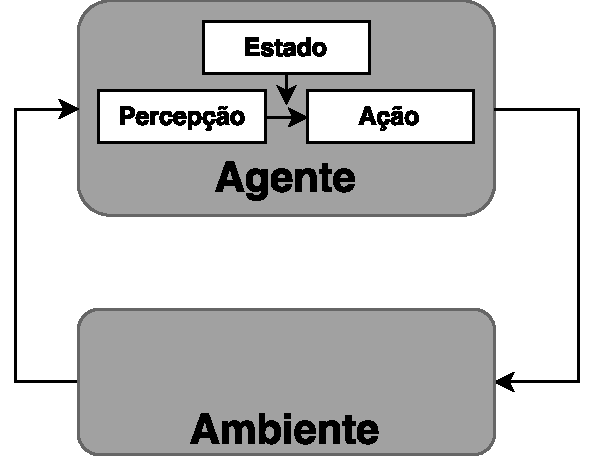
\includegraphics[width=0.4\textwidth]{fig/agentModel.pdf}
	\caption{Arquitetura de agentes com estados.}
	\label{fig:agenteModelbased}
\end{figure} 

Este tipo de arquitetura é eficaz para ambientes parcialmente observáveis, pelo fato de que o estado pode guardar informações relevantes para o agente \cite{intelligence2003modern}. No exemplo de conhecer as cidades, se guardar as visitas antigas, pode ajudar a não visitar novamente cidades que já tiverem sido visitadas. 

Dependendo do intuito do agente, conhecer o estado atual do ambiente não é suficiente. Além de estado, o agente pode precisar de uma informação para saber onde ele quer chegar, ou seja, um objetivo. Um objetivo é usado para descrever o que o agente está almejando alcançar. Para o agente conseguir alcançar o objetivo com uma melhor performance pode ser utilizado uma função de utilidade, nesta função é medido o "desejo" do agente em tomar determinada ação. Cada ação exercida pelo agente terá influência no valor de utilidade obtido \cite{intelligence2003modern}. Seguindo no exemplo, o objetivo pode ser visitar todas as cidades e a função de utilidade pode medir a distância entre as cidades, e assim podendo alcançar o objetivo com a menor distância percorrida. 



%A definição \frm{Que definição? Eu não vi nada falando de definição...} acima é uma forma geral de descrever um agente: um agente recebe um estimulo do ambiente com seus sensores e retorna uma ação por meio de seus atuadores. 
%Existem diferentes tipos de arquiteturas de agentes que acrescentam detalhes à forma geral de definir agentes. 
%Cada tipo de arquitetura combina componentes diferentes para gerar as ações \cite{intelligence2003modern}. Os quatro tipos básicos de arquiteturas de agentes, que englobam as principais características de agentes são \cite{intelligence2003modern}: 
%
%\begin{itemize}
%	\item agentes simples de reflexo (\emph{simple reflex agents});
%	\item agentes de reflexo baseados em modelo (\emph{model-based reflex agents});
%	\item agentes baseados em objetivo (\emph{goal-based agents}); e
%	\item agentes baseados em utilidade (\emph{utility-based agents}). \frm{Termos em língua estrangeira, sempre em itálico.}
%\end{itemize}  
%
%\subsection{Simple reflex agents}
%\todo[inline,color=red!80]{Tu só reorganizou as frases do livro (e traduziste alguns conceitos meio torto ``occur even in more complex environments'' $\rightarrow$ ``ambientes de alta complexidade'')!! Isto tem que ter vindo do teu entendimento!! Parei de ler no meio quando notei as similaridades com o Russel e Norvig. Repense estas seções, talvez valha a pena comprimir isto.}
%A arquitetura considerada a mais simples é a de agentes simples de reflexo. 
%Esses agentes escolhem suas ações baseados na percepção atual vinda do ambiente, ignorando qualquer outra percepção que já tenha sido observada~\cite{intelligence2003modern}. 
%A Figura~\ref{fig:agenteSimple}\frm{Coloque as figuras em uma escala adequada.} ilustra esse tipo de arquitetura. \frm{Mexi de novo na (figura $\rightarrow$ Figura) e no \emph{ilustra}, não vou mexer mais e deixo isto contigo.}
%
%\begin{figure}[ht]
%	\centering
%	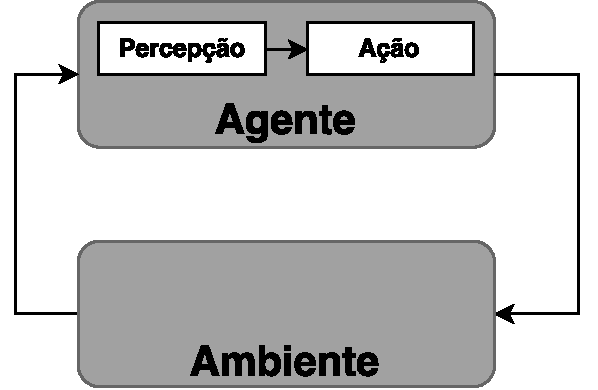
\includegraphics[width=0.4\textwidth]{fig/agentSimple.pdf}
%	\caption{Simple reflex agents}
%	\label{fig:agenteSimple}
%\end{figure} 
%
%\frm{Essa, esse, esse, essa}
%Essa arquitetura pode ser usada em ambientes de alta complexidade\frm{?!?!?!?}, como por exemplo, em carros que são dirigidos por agentes, quando o carro da frente freia, o agente deve frear também para não ocasionar em uma batida. \frm{Sério? Por que isto me parece uma afirmação contra a intuição. Tu tens que explicar isto.} 
%Esse agente utiliza uma regra de ação condicional, se acontecer uma freada no carro da frente então eu devo frear também. 
%Este tipo de agente tem a propriedade de ser simples, mas com isso sua inteligencia fica limitada \cite{intelligence2003modern}
%
%\frm{Citando muito livros!! Tentar usar a fonte original, e quando citar livro, incluir o capítulo.}.
%
%Essa abordagem é eficaz somente se o ambiente for completamente observável, ou seja, os sensores do agente tem acesso a todas as informações do ambiente a qualquer instante de tempo para detectar aspectos que são relevantes para a escolha das ações, por exemplo, um agente precisa se locomover de uma cidade para a outra, se o ambiente é completamente observável o agente consegue ver todas as estradas que chegam a cidade destino, já se o ambiente for parcialmente observável, pode ter alguma estrada que o agente não consiga ver, e se o agente não consegue ver nenhuma estrada o ambiente é não observável \cite{intelligence2003modern}. 
%
%\frm{Mega frase com diversas linhas de pensamento. Separar as idéias}
%
%\subsection{Model-based reflex agents}
%
%Os agentes de reflexos baseados em modelo utilizam um estado interno para marcar qual o estado do ambiente ele está. Este estado é utilizado como parte do processo de escolha da ação. A informação do estado pode ser de alguma informação que não pode ser obtida por alguma percepção do ambiente ou de estados que já foram visitados pelo agente. Este tipo de abordagem é eficaz para ambientes parcialmente observáveis, pelo fato de que o estado pode guardar informações relevantes para o agente \cite{intelligence2003modern}. Um modelo deste tipo de agente pode ser visto na figura \ref{fig:agenteModelbased}. 
%
%\begin{figure}[ht]
%	\centering
%	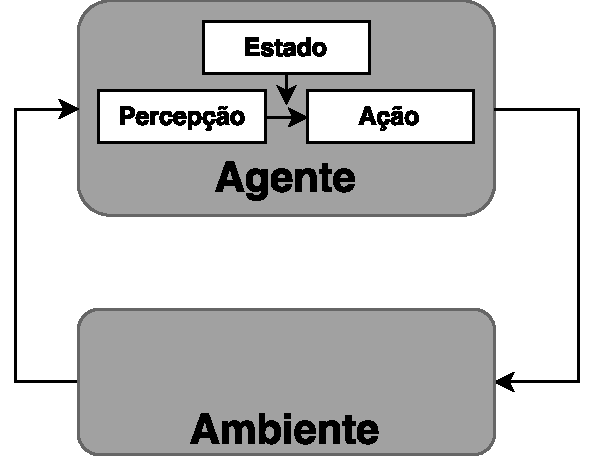
\includegraphics[width=0.6\textwidth]{fig/agentModel.pdf}
%	\caption{Model-based reflex agents}
%	\label{fig:agenteModelbased}
%\end{figure} 
%
%\subsection{Goal-based agents}
%
%Conhecendo o estado atual do ambiente, as vezes, não é suficiente para saber o que fazer \cite{intelligence2003modern}. Além do estado atual, o agente pode precisar de uma informação para saber a onde ele quer chegar, ou seja, um objetivo para descrever o que o agente está buscando alcançar. O objetivo pode ser alcançado com uma ação, outras vezes é mais complicado e leva várias ações. Esta arquitetura é diferente das outras duas apresentadas, pelo fato de se preocupar com o futuro. Para achar a sequencia de ações que alcança o objetivo pode ser usado Busca ou Planejamento, que são sub áreas da IA que tem como objetivo achar a sequencia de ações que levem o agente para o objetivo \cite{intelligence2003modern}. A figura \ref{fig:agenteGoal} mostra a arquitetura e como o objetivo influencia na escolha da ação. 
%
%\begin{figure}[ht]
%	\centering
%	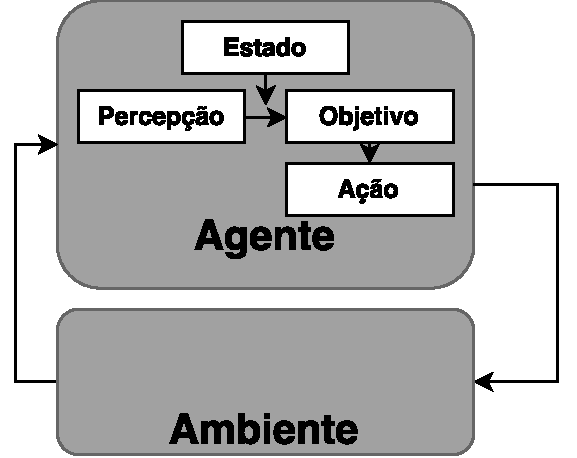
\includegraphics[width=0.6\textwidth]{fig/agenteGoal.pdf}
%	\caption{Goal-based agents}
%	\label{fig:agenteGoal}
%\end{figure} 
%
%\subsection{Utility-based agents}
%
%Apenas alcançar um objetivo pode não ser suficiente para alguns cenários, como por exemplo, um agente que deseja chegar a determinada cidade, existem mais de um caminho que levam para a mesma cidade, indo pelo caminho mais longo o agente ainda estará chegando no objetivo. Para o agente conseguir alcançar o objetivo com uma melhor performance é utilizado uma função de utilidade, nela é medido o "desejo" do agente em tomar determinada ação. Cada ação exercida pelo agente terá influencia no valor de utilidade obtido \cite{intelligence2003modern}. Esta arquitetura é melhor utilizada em ambientes parcialmente observáveis e estocásticos, um ambiente estocástico é onde não há conhecimento preciso do próximo estado dado determinada ação \cite{intelligence2003modern}. A figura \ref{fig:agenteUtility} representa essa arquitetura.  
%
%\begin{figure}[ht]
%	\centering
%	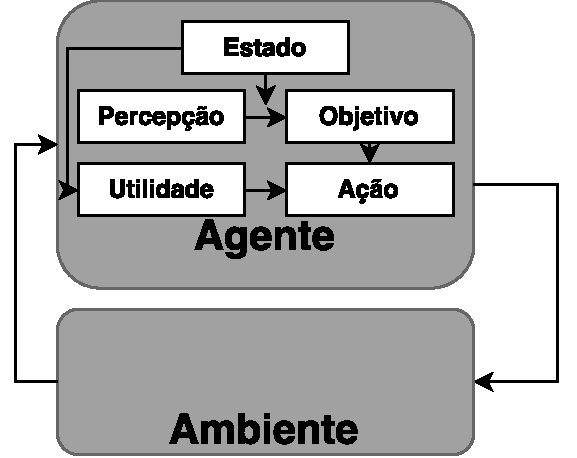
\includegraphics[width=0.6\textwidth]{fig/agentUtility.pdf}
%	\caption{Utility-based agents}
%	\label{fig:agenteUtility}
%\end{figure} 


